\chapter{Medida del rendimiento}
\label{chap:medida_rendimiento}

\lettrine{L}{a} medida del rendimiento y el resultado de la misma es una parte fundamental en la evaluación y relevancia de un supercomputador, hasta el punto en el que se compite por ver cuales desarrollan un mejor resultado\footnote{\url{https://www.top500.org}}.

En este caso, si bien el rendimiento no es una prioridad, es conveniente realizar estas pruebas, especialmente para poder observar el impacto que tiene la red de comunicaciones entre los núcleos de una sola CPU, o entre múltiples CPUs y memorias. En resumen, medir la escalabilidad, que como se observa en \nameref{sec:comparacion_resultados} no es en absoluto espectacular.

\section{NAS Parallel Benchmarks}
Los \acrlong{npb} (\acrshort{npb})\footnote{\url{https://www.nas.nasa.gov/software/npb.html}} son una \textit{suite} de tests diseñados por la División de Supercomputación de la NASA para la medida del rendimiento de supercomputadores paralelos.

Estos benchmarks se dividen principalmente ocho benchmarks, teniendo otras adaptaciones para diferentes paradigmas de computación paralela, como puede ser de paralelización híbrida, computación desestructurada, o mallas de computación.

A su vez cada benchmark tiene múltiples clases, siendo estas \texttt{S, W, A, B, C, D, E}, y representando cada una un nivel de requerimientos superior, respectivamente. Específicamente, la las clases A, B y C suponen cuadruplicar el tamaño con respecto a la anterior, y las D, E y F (para los benchmarks que tienen estas clases disponibles), multiplican por 16 el tamaño del anterior.

En este caso se empleará la clase C para todos los benchmarks, excepto en MG que será clase B, y FT, que será clase A debido a limitaciones de memoria en los nodos.

\subsection{Clases y procesos}
Los benchmarks a ejecutar serán \texttt{LU, CG, FT, IS, MG y EP}, es decir, se excluyen \texttt{BT, SP y DT}. Esto es así debido a que los dos primeros requieren un número cuadrado perfecto de procesos, por lo que solo se podría ejecutar en 1, 4, 9, 16\dots procesos, y medir su rendimiento sería extraño debido a lo desbalanceado del mismo. En cuanto a DT, requiere una cantidad mínima de procesos en función de la clase del problema, procesos que para clase A y superior no son suficientes, por lo que se ha optado por descartarlo.

En concreto, los requerimientos para el número de procesos son los siguientes\footnote{Contenidos del fichero \texttt{README.install} en \texttt{NPB3.4-MPI}}:

\begin{lstlisting}
Different benchmark has different requirement for process count,
as listed below:

  BT, SP         - a square number of processes (1, 4, 9, ...)
  LU             - 2D (n1 * n2) process grid where n1/2 <= n2 <= n1
  CG, FT, IS, MG - a power-of-two number of processes (1, 2, 4, ...)
  EP, DT         - no special requirement
\end{lstlisting}

\subsection{Metodología}
La metodología es una muy importante parte en cualquier medida y análisis de la realidad, ya que permite filtrar y categorizar datos como más o menos fidedignos. En este caso la metodología a seguir ha sido moderadamente sencilla.

Se han realizado 5 ejecuciones de todos los problemas clase C, y 9 ejecuciones de los clase A o B. Esto es así, ya que a menor tiempo de ejecución, mayor probabilidad de obtener un dato atípico. Por suerte, y muy probablemente debido a la instalación mínima del sistema operativo, no ha habido variaciones significativas entre ejecuciones.

Los resultados de los benchmarks pueden encontrarse anexados en TODO \#REF\# VALUES.

\subsection{Prerrequisitos}
Para poder realizar las medidas de rendimiento, primero se necesitan tanto las herramientas de compilación como las de ejecución. Estas dependencias se deben satisfacer ejecutando:

\begin{lstlisting}[language=bash]
# Se añade la opción --needed debido a que hay paquetes del metapaquete base-devel que ya están instalados, y no es necesario reinstalar.
# Tras ejecutar el comando se aceptan las opciones por defecto
pacman -S base-devel openmpi gcc-fortran wget --needed
\end{lstlisting}

\subsection{Instalación de los \acrshort{npb}}
A continuación se deben descargar, configurar, y compilar los \acrlong{npb} únicamente en el nodo maestro. Esto se realizará como \texttt{mpiuser} en la carpeta \texttt{/mpishared} de la siguiente forma:

\begin{lstlisting}[language=bash]
# Descarga de la última versión de NPB (3.4.2)
wget https://www.nas.nasa.gov/assets/npb/NPB3.4.2.tar.gz

# Descomprimir el archivo descargado
tar xzfv NPB3.4.2.tar.gz

# Y entrar en la versión de los NPB con MPI
cd /mpishared/NPB3.4.2/NPB3.4-MPI

# Copiar los archivos de configuración para la compilación
#  1- Para el archivo make.def se añaden un par de argumentos a los flags de compilación:
#   1.1- -fallow-argument-mismatch Esto permite que el código compile en las últimas versiones de gfortran
#   1.2- -march=native Optimiza para la arquitectura específica de rpi4
sed 's/^FFLAGS\s*=\s*-O3/FFLAGS  = -O3 -fallow-argument-mismatch -march=native/g' config/make.def.template | sed -e 's/^CFLAGS\s*=\s*-O3/CFLAGS  = -O3 -march=native/g' > config/make.def

#  2- Para el archivo suite.def se hace que todos los tests sean clase C menos FT, que por razones de memoria es clase A, y MG clase B, por los mismos motivos.
sed 's/S$/C/g' config/suite.def.template | sed -e 's/ft\s*C$/ft\tA/g' | sed -e 's/mg\s*C$/mg\tB/g' > config/suite.def

# Finalmente se compilan todos los tests con make suite (con todas las CPU en paralelo)

# TODO REMOVE CLOSING DOLLAR FOR LATEX SYNTAX $
make suite -j4
\end{lstlisting}

\subsection{Preparativos para la ejecución de los benchmarks}
Para la ejecución de los benchmarks de forma paralela se necesita algún método para coordinar la ejecución del programa en todos los nodos.

\begin{itemize}
    \item Para un solo nodo con múltiples núcleos es sencillo, ya que comparten memoria, usuarios y almacenamiento
    \item Para múltiples nodos sin embargo es algo más complejo. Como ya se menciona en las Subsecciones \ref{ssec:gen_ssh} y \ref{ssec:serv_nfs}, es necesario disponer de:
    \begin{itemize}
        \item Almacenamiento compartido en forma de NFS para alojar los ejecutables
        \item Autenticación y gestión común para el lanzamiento de los programas paralelos en forma de SSH con par de claves
    \end{itemize}
\end{itemize}

A MPI se le indica qué nodos deben ejecutar las tareas mediante un archivo de hosts, o \textit{hostsfile}\cite{mpi_hostfile_option}. Este fichero contiene las direcciones de los diferentes computadores que componen el cluster, así como el número de tareas que pueden ejecutar (habitualmente coincidente con su número de núcleos)

Así, se crea en \texttt{/mpishared} el fichero \texttt{hostfile} con los hostname de todos los nodos:

\begin{lstlisting}[language=bash]
rpi0 slots=4
rpi1 slots=4
rpi2 slots=4
rpi3 slots=4
rpi4 slots=4
rpi5 slots=4
rpi6 slots=4
rpi7 slots=4
\end{lstlisting}

\subsection{Ejecución de los benchmarks}
Ejecutar los benchmarks es moderadamente sencillo: \texttt{mpirun} funciona de la siguiente forma <TODO (posiblemente sección MPI) insertar explicación detallada> (posiblemente reubicar)

La ejecución de cada uno de los benchmarks se realizará mediante el siguiente comando \textbf{como usuario mpiuser}, en el que se debe especificar el número de procesos a crear.\footnote{Se añade \texttt{--mca opal\_warn\_on\_missing\_libcuda 0} para evitar una advertencia que no interesa en la salida por pantalla}

\begin{lstlisting}[language=bash]
mpirun -np <NUM_PROCS> --hostfile /mpishared/hostfile --mca opal_warn_on_missing_libcuda 0 /mpishared/NPB3.4.2/NPB3.4-MPI/bin/<KERNEL>.<CLASS>.x
\end{lstlisting}

Como estos parámetros son fijos, es posible scriptear la ejecución de los benchmarks, así como la recolección de resultados, siempre y cuando solamente exista una clase por benchmark:

\begin{lstlisting}[language=bash]
#!/bin/sh

mkdir -p "results"

BENCHMARKS=( lu cg ft is mg ep )
MPIRUNFLAGS="--mca opal_warn_on_missing_libcuda 0"

for i in "${BENCHMARKS[@]}"
do
    for j in 1 2 4 8 16 32
    do
        mpirun -np $j --hostfile /mpishared/hostfile $MPIRUNFLAGS /mpishared/NPB3.4.2/NPB3.4-MPI/bin/${i}.*.x | tee -a results/$i.$j.run
    done
done
\end{lstlisting}

Ante diferentes números de procesos, \acrshort{mpi} elige la configuración más óptima, intentando mantener siempre las CPUs lo más cerca posible.

\section{Comparación de Resultados}
\label{sec:comparacion_resultados}
La comparación de resultados es precisamente el objetivo de los benchmarks. En este caso interesa medir la escalabilidad del cluster, y no compararlo contra otros. Esto es, medir la eficacia con la que, aumentando los recursos computacionales aumenta el rendimiento en la misma medida.

Se muestran a continuación los datos expresados en MOPS (\textbf{M}ega/\textbf{M}illion \textbf{O}perations \textbf{P}er \textbf{S}econd). En función de si estas operaciones son en punto flotante o no, también se podrán llamar \acrshort{mflops} (\textbf{M}ega/\textbf{M}illion \textbf{FL}oating point \textbf{O}perations \textbf{P}er \textbf{S}econd).

\subsection{CG}
CG blabla TODO

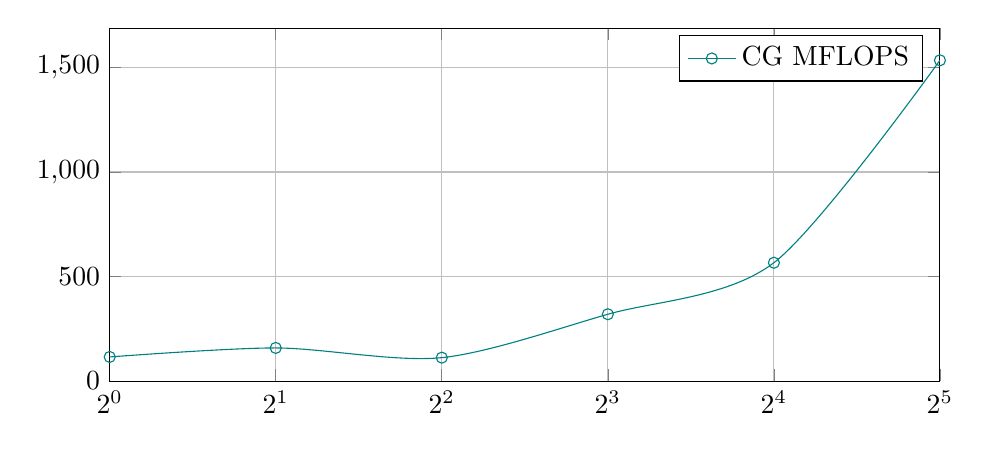
\begin{tikzpicture}
\begin{axis}[
    xmin = 1, xmax = 32, xmode=log, log basis x=2,
    ymin = 0,
    width = \textwidth,
    height = 0.5\textwidth,
    grid=both,
]
\addplot[teal,smooth,mark=o] coordinates {
    (1,115.37)
    (2,158.44)
    (4,112.03)
    (8,319.65)
    (16,565.98)
    (32,1534.13)
};
\legend{CG MFLOPS};
\end{axis}
\end{tikzpicture}

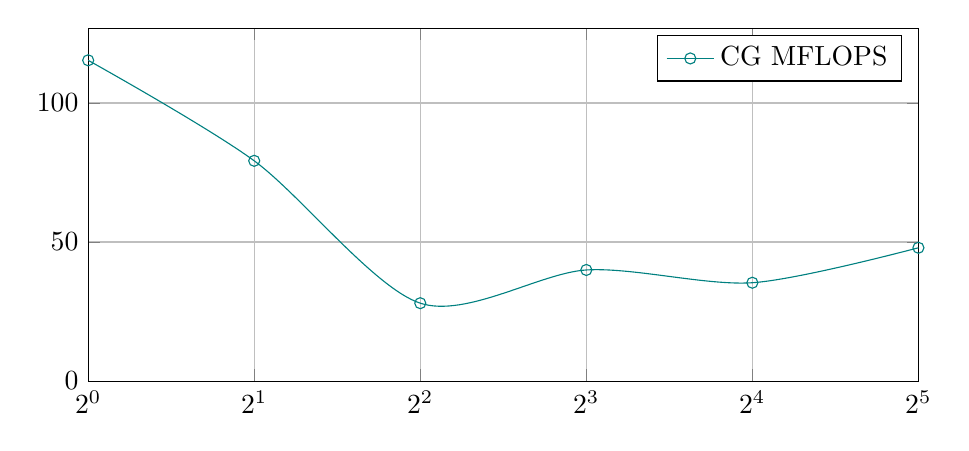
\begin{tikzpicture}
\begin{axis}[
    xmin = 1, xmax = 32, xmode=log, log basis x=2,
    ymin = 0,
    width = \textwidth,
    height = 0.5\textwidth,
    grid=both,
]
\addplot[teal,smooth,mark=o] coordinates {
    (1,115.37)
    (2,79.22)
    (4,28.01)
    (8,39.96)
    (16,35.37)
    (32,47.94)
};
\legend{CG MFLOPS};
\end{axis}
\end{tikzpicture}
